\section{Optimisation of Pooled Funds Investment Strategies}

So far, we have managed to test two different strategies. We have analysed their return and risk in a simulated scenario, within the context of a pension plan. In order to assess the risk of the strategies, so far we have been measuring the market risk of the investment, by computing the \emph{Expected Shortfall}. However, in real-scenario pension plans, there are plenty of other risks that should be taken into consideration. One important risk, not rarely underestimated, is the so-called \textbf{Longevity Risk}. Longevity risk is referred to the probability of retirees that will live longer than expected and will thus exhaust all their savings, and all the costs incurred. This risk might doom some individuals to utter poverty or to burden relatives.

Recently, two worldwide phenomena ought to be highlighted. The collapse in low-risk assets returns as government bonds or blue chip stocks. And the observed demographic transition~\textcite{b:demographic, a:bongaarts-human}, in which both birth rates and death rates are plumbing down; increasing the life expectancy of elder individuals. The combination of these two factors is leading to an increase in longevity risk that pension plans providers are facing, rising pension premiums and stagnating disposable incomes by savers and pushing them to work longer years before retirement.

As a response to this challenge, the work of~\cite{a:donnelly-transparency} and \cite{a:brautigam-pool} suggested a different approach to face longevity risk, the concept of \textbf{Pooled Funds}.

Pooled Funds are funds formed by many different individual savers that aggregate their savings together. The main characteristic of Pooled Funds is the fact that it takes into account the survival rate of the savers. Sadly, not all investors live long enough to cash back the profits of their investments. Pooled Funds make a strength out of this and proportionally redistributes the invested money of the deceased among the rest of the investors. Alongside other advantages, pooled funds benefit from economies of scale, cheaper diversification and a more efficient management of longevity risk.

In this section we will study the application of both CPPI and Alternative schemes that we have developed in previous sections under the framework of a simplified pooled fund.

\subsection{Simulating the Pooled Fund}

In order to simulate the pooled fund, we will construct a simple scenario where many investors of the same age start investing at the same time. We will take real death probabilities at each age, and we will simulate the death of some of the savers.

When savers die, some proportion $w$ of their saved money stays in the pool, benefiting the survivors. The rest is extracted from the pool, to their family or inheritors. In order to simulate the probability of death for each individual, we took the empirical measures of death probability for every age from the Spanish Government~\cite{o:mortality-table}. This way, we can assume that from a starting number of persons $n$ of the same age, and thus with the same death probability $p$, the number of persons that would die $X$ before the next year should follow a \emph{Binomial Distribution}. Thus the probability of $k$ deaths is:

\begin{align}
  Pr(X = k) = \frac{n!}{k!(n-k)!} p^k (1-p)^{n-k} \emph{.}
\end{align}

Now we can now make use of the algorithm described in \cite{a:schmeiser-binomial} to generate random numbers $k$ that follow a Binomial Distribution, and assume those $k$ to be the simulated deaths for the following year. Once we have $k$, we can compute how much proportional wealth $M$ has been given to every investor of the common pool by:

\begin{align}
  M = \frac{k}{n}w \emph{.}
\end{align}

The point of constructing the Pooled Fund in such a way, is that we are not altering the core principles of the assumptions taken building the Alternative Model. The relative proportion $\pi$ of wealth to be allocated in risky assets remains untouched, we are just altering the $x = X(t)$ present in  Equation~\ref{eq:maxE}. Resulting in

\begin{align}
	\max_{\pi}\EX\giventhat{u_{X(T)}}{x(1 + M)} \emph{.}
\end{align}

And thus the wealth of the investor will behave as

\begin{align}
	dX = \alpha \pi(t)X(t)dt + \sigma \pi(t)X(t)dW(t) + dC(t) + dM(t)X(t)w \textit{.}
\end{align}

In the snippet in Appendix~\ref{ap:mort-code} we show the necessary R code to perform this simulation for both CPPI and Alternative schemes.

\subsection{Results}

Now we are going to replicate the measures taken in the previous section but with the added condition of mortality and see whether or not the differences spotted between the CPPI and the Alternative strategies remain similar.

Firstly, we plot together the frequency histograms for the final wealth distribution for
both models.

\begin{figure}[h]
    \centering
    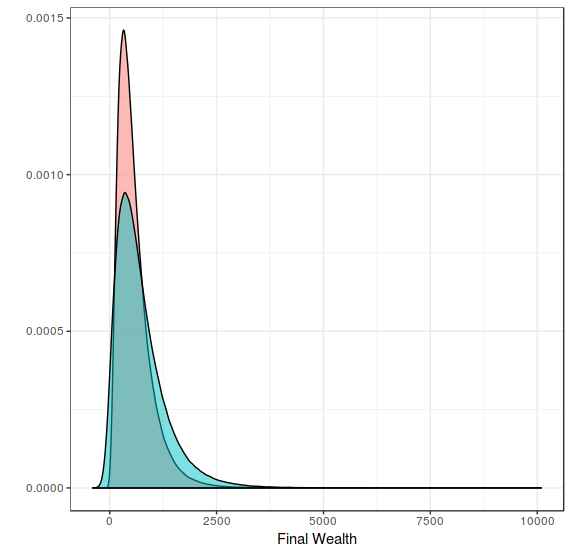
\includegraphics[scale=0.75]{./images/mort_final_wealth.png}
    \caption{Results of $1,000,000$ simulations for the both models with mortality. Final wealth obtained for every simulation. The blue one is the CPPI, and the red one is the Alternative. With $\pi = 0.5$, $\alpha = 0.343$, $\sigma = 0.1544$, $a = 10$, $T = 60$, $A = 0.5$.}
    \label{fig:mort_fw}
\end{figure}


Looking at Figure \ref{fig:mort_fw} we might note that the results are quite similar. Nevertheless, we can spot some differences in the shape of the non-central zones of the figure, where the Alternative Strategy seems to show less dispersion.

With a quick glimpse at Figure \ref{fig:mort_loss} we can already notice the great difference in the loss distribution of both schemes. It is clear that the CPPI is far more risky than the Alternative.

\begin{figure}[h]
    \centering
    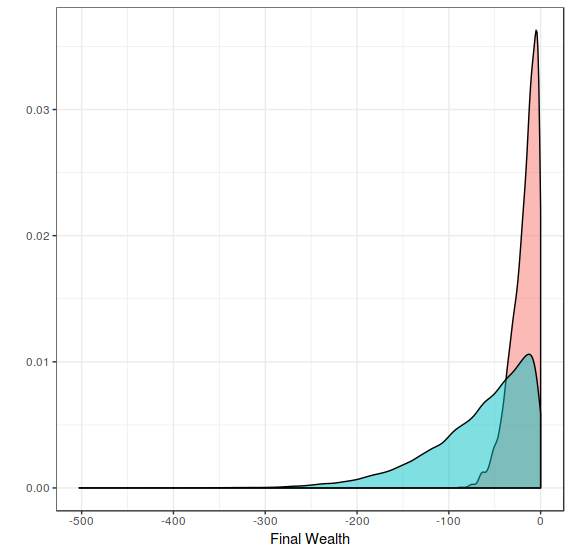
\includegraphics[scale=0.75]{./images/loss_both_mort.png}
    \caption{Results of $1,000,000$ simulations for the both models with mortality. Losses obtained for every simulation. The blue one is the CPPI, and the red one is the Alternative. With $\pi = 0.5$, $\alpha = 0.343$, $\sigma = 0.1544$, $a = 10$, $T = 60$, $A = 0.5$.}
    \label{fig:mort_loss}
\end{figure}

Since the conclusions extracted from just one value of $\pi$ may be misleading, let us iterate these simulations for many values of $\pi$ and $K$. In order to equalise the level of risk of the result of both strategies, we ought to make use of Formula \ref{eq:kes}, as we have done before. The problem is that we can not be sure that the assumptions and deduction from~\cite{a:guillen-optimisation} will be standing for this scenario that we are constructing. In fact, looking at the results of Figure~\ref{fig:es-es_mort} we can be sure that the measured Expected Shortfall are not the same for both strategies when in a Pooled Fund.

\begin{figure}
    \centering
    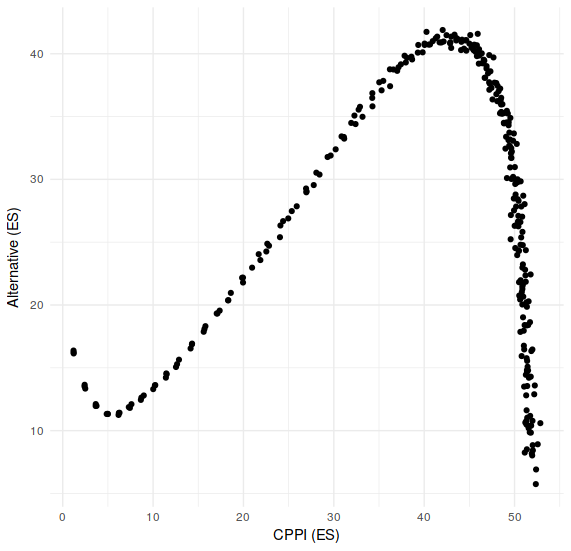
\includegraphics[scale=0.5]{./images/es-es.png}
    \caption{Expected Shortfall measured from the results of $100,000,000$ simulations for the both models with mortality. With  many values for $\pi$, $A$ and $K$; $\alpha = 0.343$, $\sigma = 0.1544$, $a = 10$, $T = 60$ and $A = 0.5$.}
    \label{fig:es-es_mort}
\end{figure}

In order to pursue further results, the necessary value of $K$ in order to ensure equal Expected Shortfall for both strategies has been found numerically, whose results are shown in Figure~\ref{fig:pi-a_mort}, Figure~\ref{fig:es-es_mort} and Table~\ref{tab:cppi_alt_mort}.


\begin{table}[h]
\centering
\caption{Results of $100,000$ simulations of both CPPI and Alternative models in a Pooled Fund, using different risk levels, with $\alpha = 0.343$, $\sigma = 0.1544$, $a = 10$, $T = 60$, $A = 0.5$.}
\label{tab:cppi_alt_mort}
\begin{tabular}{ccccccc}
\textbf{$\pi$} & \textbf{ES } & \textbf{$K$} & \textbf{CPPI ret} & \textbf{Alt ret} & \textbf{diff}  & \textbf{equiv $\pi$}\\
10  & 140.32  & 18.11 & 1.84 & 1.97 & 0.13 & 0.15 \\
20  & 88.75  & 88.41 & 2.13 & 2.79 & 0.65 & 0.34 \\
30  & 58.50  & 96.45 & 2.66 & 2.80 & 0.13 & 0.32 \\
40  & 20.85  & 165.75  & 3.13 & 3.59 & 0.46 & 0.49 \\
50  & -28.11 & 232.00  & 3.46 & 4.17 & 0.70 & 0.64 \\
60  & -73.18 & 294.04 & 3.83 & 4.67 & 0.83 & 1.06 \\
70  & -118.58 & 381.23 & 4.24 & 5.40 & 1.15 & 1.63 \\
80  & -153.69 & 424.03 & 4.77 & 5.85  & 1.07 & *                 \\
90  & -223.58 & 524.09 & 4.88 & 6.77 & 1.88 & *                 \\
100 & -261.12   & 618.38 & 5.16 & 6.79 & 1.62 & *

\end{tabular}
\end{table}


% The Pooled Fund has the effect of the wealth of all savers to increase dramatically. In fact, for lower risk levels as for $\pi < 0.5$, the final wealth of all simulations is so huge that the Expected Shortfall happenes to result positive and utterly large, instead of negative. So in order for the Alternative Strategy to equal that Expected Shortfall, the Formula \ref{eq:the_formula} leads to so hugely negative value of $K$ that the $\pi$ comes negative. Implying a short position in the market. Akwnoledging the non-sense that could derive from that decision, we have decided to cast out those simulations and simply state that this equivalence between the Expected Shortfall of both strategies is not valid for positive values of the Expected Shortfall.

As in the previous section, equivalent values of $\pi$ have been working as a succint metric to compare the performance of this two strategies, taking into account both return and risk. Hence, as long as the equivalent $\pi$ remains above than the initial $\pi$, we can say that the Alternative Strategy is outperforming
the CPPI. Which is clear for most of the values of initial $\pi$ and a fixed value for $A$. Additionally, we can expand this results and find the iterated simulation of Table \ref{tab:cppi_alt_mort} for many values of $A$, as shown in Figure~\ref{fig:pi-a_mort}.

% \begin{figure}[h]
%     \centering
%     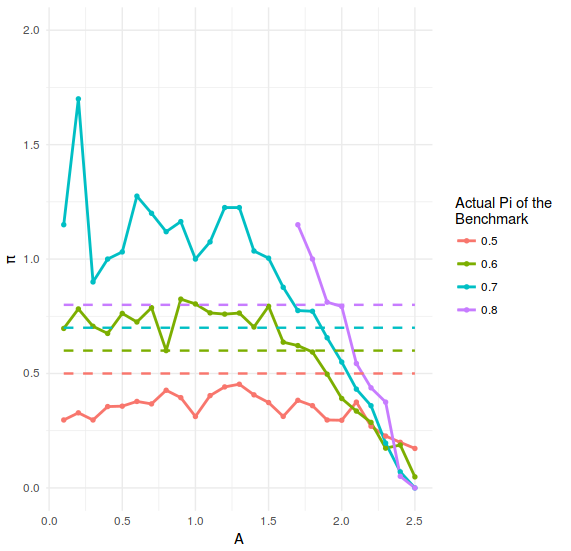
\includegraphics[scale=0.75]{./images/pi-A_mort_2.png}
%     \caption{Plot that shows the relation between equivalent $\pi$ and $A$, for many different initial $\pi$. From the results of $100,000$ simulations for each curve, with $\alpha = 0.343$, $\sigma = 0.1544$, $a = 10$, $T = 60$.}
%     \label{fig:pi-a_mort}
% \end{figure}

\begin{figure}
\centering
\begin{subfigure}{.5\textwidth}
    \centering
    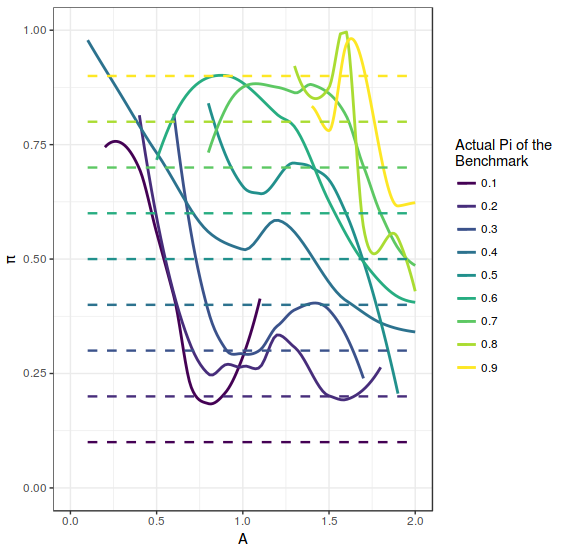
\includegraphics[scale=0.5]{./images/pi-a_mort2.png}
    \caption{Plot that shows the relation between equivalent $\pi$ and $A$.}
    \label{fig:pi-a_mort}
\end{subfigure}%
\begin{subfigure}{.5\textwidth}
    \centering
    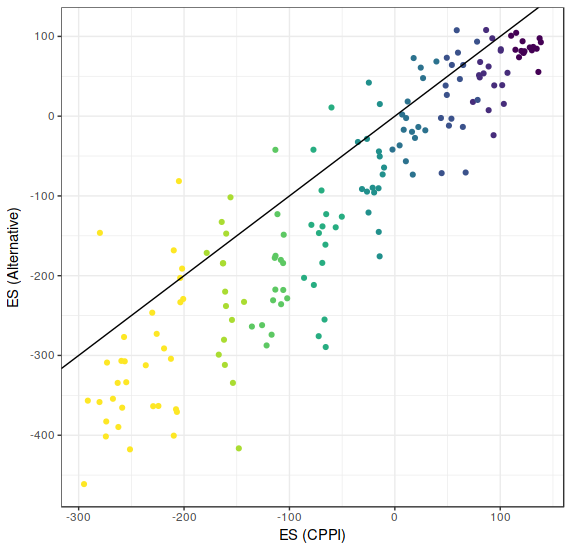
\includegraphics[scale=0.5]{./images/es-es_mort_2.png}
    \caption{Scatterplot that shows the equivalence between the Expected Shortfall derived from the simulations of Figure \ref{fig:pi-A_all-pis2}.}
    \label{fig:es-es_mort}
\end{subfigure}
\caption{Results from $20,000,000$ simulations performed for many different values of $\pi$ and $A$, with $\alpha = 0.343$, $\sigma = 0.1544$, $a = 10$, $T = 60$.}
\label{fig:compare_mort}
\end{figure}

The main difference we can note between Figure \ref{fig:es-es_pi} and Figure \ref{fig:es-es_mort_2} is that the equivalence between Expected Shortfall tends to be true, but is far more volatile in the case of a Poolued Fund. This leads to far more disperse result in Figure~\ref{fig:pi-a_mort} than in Figure~\ref{fig:pi-A_all-pis2}. Despite that, we can glimpse some patterns within the results that let us observe some distinctions between the results without and with mortality. Note that the values that are not present in the plot of Figure~\ref{fig:pi-a_mort} is because there were not value of equivalent $\pi$ for the CPPI capable of equaling the results of the Alternative. Note also that this happens more often for higher values of $\pi$.

Attending at the obtained results, we can see that outside of a Pooled Fund, the decision of whether the CPPI strategy or the Alternative are more worth it, has to do with the value of $A$ alone, not with $\pi$. On the contrary, within the context of a Pooled Fund, we can see that the Alternative model shines over the CPPI for higher values of $\pi$. In fact, for higher values of $\pi$, the Alternative strategy outperforms the CPPI so much that often an equivalent value $\pi_b$ for the CPPI to equal the return of the Alternative simply does not exist. This result is of great importance, specially considiering that both strategies incurr in the same risk level, as it is shown in Figure~\ref{fig:es-es_mort}.

As before, we can roughly observe a downhill behaviour of the plot.  This trend indicates that, for higher levels of $A$, where $A$ is interpretd as the inverse of the risk aversion, the Alternative strategy tends to be less relatively worth it, compared to the CPPI. Nonetheless, we should highlight a sweetspot around $A = 1.5$ where the plot gets to relative maximum for many levels of $\pi$.




